%!TEX root = <main.tex>
\section{Incremental Inference Optimizations}\label{sec:exact}
We start with a theoretical characterization of how much speedups one can expect from incremental inference for OBE. We then dive into our novel algebraic framework that enables incremental inference for CNN layers and integrates it multi-query optimization for OBE.

%inspired by incremental view maintenance in relational databases~\cite{ivm}. We start with a theoretical characterization of how much speedup is possible to set the expectation. We then dive into our novel algebraic framework to enable and optimize incremental inference for OBE. To the best of our knowledge, ours is the first work to combine incremental view maintenance with multi-query optimization for repeated CNN inference.

\subsection{Expected Speedups}
The basic reason why incremental view maintenance (IVM) for relational queries offers speedups is that when a part of the input relation is updated, IVM only computes the part of output that gets changed. We bring the IVM notion to CNNs with CNN layers being our ``queries'' and materialized feature tensors being our ``relations.'' OBE updates only a part of the input; so, only some parts of the output tensors need to be recomputed. We create an algebraic framework to determine which parts these are for a CNN layer (Section 3.2) and how to propagate updates across layers (Section 3.3). Given a CNN $f$ and the occlusion patch, our framework can determine using ``static analysis'' over $f$ how many FLOPs can be saved. This let us derive an upper bound on the possible speedup--we call this the ``theoretical speedup.''

More precisely, let the output tensor dimensions of layer $l$ be $(C_{\mathcal{O}:l} , H_{\mathcal{O}:l} , W_{\mathcal{O}:l})$. An incremental update recomputes a smaller local spatial context with width $W_{\mathcal{P}:l} \le W_{\mathcal{O}:l}$ and height $H_{\mathcal{P}:l} \le H_{\mathcal{O}:l}$. Thus, the computational cost of incremental inference for layer $l$, $Q_{inc:l}$, and the total computational cost for incremental inference for $f$, $Q_{inc}$, are given by Equations~(\ref{eqn:inc_local}) and ~(\ref{eqn:inc_all}).

\begin{align}
\label{eqn:inc_local}
Q_{inc:l} =&~ (C_{\mathcal{I}:l} \cdot H_{\mathcal{K}:l} \cdot W_{\mathcal{K}:l})  (C_{\mathcal{O}:l} \cdot H_{\mathcal{P}:l} \cdot W_{\mathcal{P}:l})\\
\label{eqn:inc_all}
Q_{inc} =&~ \sum_{l~\mathit{in}~f} Q_{inc:l}
\end{align}

The above costs can be much smaller than $Q_{:l}$ and $Q$ in Equations~(\ref{eqn:full_local}) and~(\ref{eqn:full_all}) earlier.
The \textit{theoretical speedup} is defined as the ratio $\frac{Q}{Q_{inc}}$. It tells us how beneficial incremental inference can be in the best case \textit{without} performing the inference itself. It depends on several factors: the occlusion patch size, its location, the parameters of layers (kernel dimensions, stride, etc.), and so on. Calculating it is non-trivial and requires careful analysis, which we perform. The location of patch affects this ratio because a patch placed in the corner leads to fewer updates overall than one placed in the center of the image. Thus, the ``worst-case'' theoretical speedup is determined by placing the patch at the center.

We performed a sanity check experiment to ascertain the theoretical speedups for a few popular deep CNNs. For varying occlusion patch sizes (with the same stride of 1), we plot the theoretical speedups of different deep CNNs in Figure~\ref{fig:redundancy_ratio} shows the results. VGG-16 has the highest theoretical speedups, while DenseNet-121 has the lowest. Most CNNs fall in the 2X--3X range. The differences arise due to the specifics of the CNNs' architectures: VGG-16 has small Convolution filter kernels and strides, which means full inference incurs a high computational cost ($Q = 15$ GFLOPs). In turn, incremental inference is most beneficial for VGG-16. Note that we assumed an image size of $224 \times 224$ for this plot; if the image is larger, the theoretical speedups will be higher.

While one might be tempted to think that speedups of 2X-3X may not be ``that significant'' in practice, we find that they indeed are significant for at least two reasons. First, \textit{users often wait in the loop} for OBE workloads for performing interactive diagnoses and analyses. Thus, even such speedups can improve their productivity, e.g., reducing the time taken on a CPU from about 6min to just 2min, or on a GPU from 1min to just 20s. Second, and equally importantly, incremental inference is the \textit{foundation for our approximate inference} optimizations (Section 4), which amplify the speedups we achieve for OBE. For instance, the speedup for Inception3 goes up from only 2X for incremental inference to up to 8X with all of our optimizations enabled. Thus, incremental inference is critical to optimizing OBE.

\begin{figure}[t]
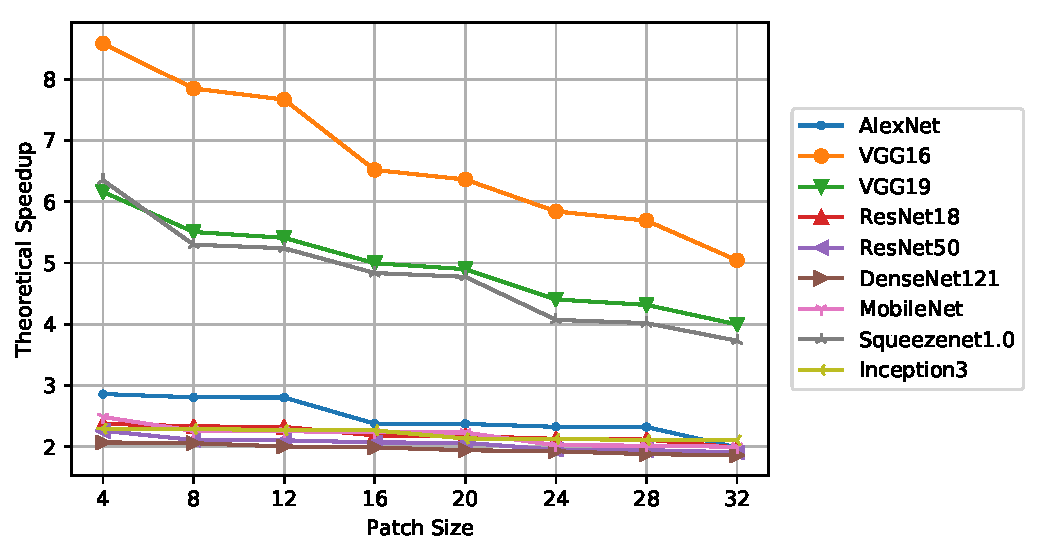
\includegraphics[width=\columnwidth]{images/redundancy_ratio}
\vspace{-8mm}
\caption{Theoretical speedups for popular deep CNN architectures with incremental inference.}
\label{fig:redundancy_ratio}
\end{figure}


\subsection{Single Layer Incremental Inference}\label{sec:inc_computation}
We now present our algebraic framework for incremental updates to the materialized output tensor of a CNN layer. As per the discussion in Section 2.2, we focus only on the non-trivial layers that operate at the granularity of a local spatial context (Convolution and Pooling). We call our modified version of such layers ``incremental inference operations.''

\vspace{2mm}
\noindent \textbf{Determining Patch Update Locations.} We first explain how to calculate the coordinates and dimensions of the \textit{output update patch} of layer $l$ given the \textit{input update patch} and layer-specific parameters. Figure~\ref{fig:dimensions} presents a simplified illustration of these calculations. Our coordinate system's origin is at the top left corner. The input update patch is shown in red/dark color and starts at $(x^\mathcal{I}_{\mathcal{P}:l}, y^\mathcal{I}_{\mathcal{P}:l})$, with height $H^\mathcal{I}_{\mathcal{P}:l}$ and width $W^\mathcal{I}_{\mathcal{P}:l}$. The output update patch starts at $(x^\mathcal{O}_{\mathcal{P}:l}, y^\mathcal{O}_{\mathcal{P}:l})$ and has a height $H^\mathcal{O}_{\mathcal{P}:l}$ and width $W^\mathcal{O}_{\mathcal{P}:l}$. Due to overlaps among filter kernel positions during inference, computing the output update patch requires us to read a slightly larger spatial context than the input update patch--we call this the ``read-in context,'' and it is illustrated by the blue/shaded region in Figure~\ref{fig:dimensions}. The read-in context starts at $(x^\mathcal{R}_{\mathcal{P}:l}, y^\mathcal{R}_{\mathcal{P}:l})$, with its dimensions denoted by $W^\mathcal{R}_{\mathcal{P}:l}$ and $H^\mathcal{R}_{\mathcal{P}:l}$. Table~\ref{table:optimizer_symbols} summarizes all this additional notation for this section. The relationship between these quantities along the width dimension (similarly along the height dimension) can be expressed as follows:


\begin{align}
\label{eqn:xcoordinate}
x^\mathcal{O}_{\mathcal{P}:l} =&~ max\big(\lceil (P_{x:l} + x^\mathcal{I}_{\mathcal{P}:l} - W_{\mathcal{K}:l} + 1)/S_{x:l} \rceil, 0\big)\\
\label{eqn:patchwidth}
W^\mathcal{O}_{\mathcal{P}:l} =&~ min\big(\lceil (W^\mathcal{I}_{\mathcal{P}:l} + W_{\mathcal{K}:l} - 1)/ S_{x:l} \rceil, W_{\mathcal{O}:l}\big)\\
\label{eqn:xreadcoordinate}
x^\mathcal{R}_{\mathcal{P}:l} =&~ x^\mathcal{O}_{\mathcal{P}:l} \times S_{x:l} - P_{x:l}\\
\label{eqn:readpatchwidth}
W^\mathcal{R}_{\mathcal{P}:l} =&~ W_{\mathcal{K}:l} + (W^\mathcal{O}_{\mathcal{P}:l}-1) \times S_{x:l}
\end{align}

% \begin{align}
% \label{eqn:xcoordinate}
% x^\mathcal{O}_\mathcal{P} =&~ max\big(\lceil (P_x + x^\mathcal{I}_\mathcal{P} - W_\mathcal{K} + 1)/S_x \rceil, 0\big)\\
% \label{eqn:ycoordinate}
% y^\mathcal{O}_\mathcal{P} =&~ max\big(\lceil (P_y + y^\mathcal{I}_\mathcal{P} - H_\mathcal{K} + 1)/S_y \rceil, 0\big)
% \end{align}

% \begin{align}
% \label{eqn:patchwidth}
% W^\mathcal{O}_\mathcal{P} =&~ min\big(\lceil (W^\mathcal{I}_\mathcal{P} + W_\mathcal{K} - 1)/S_x \rceil, W_{\mathcal{O}}\big)\\
% \label{eqn:patchheight}
% H^\mathcal{O}_\mathcal{P} =&~ min\big(\lceil (H^\mathcal{I}_\mathcal{P} + H_\mathcal{K} - 1)/S_y \rceil, H_{\mathcal{O}}\big)
% \end{align}

% \begin{align}
% \label{eqn:xreadcoordinate}
% x^\mathcal{R}_\mathcal{P} =&~ x^\mathcal{O}_\mathcal{P} \times S_x - P_x\\
% \label{eqn:yreadcoordinate}
% y^\mathcal{R}_\mathcal{P} =&~ y^\mathcal{O}_\mathcal{P} \times S_y - P_y
% \end{align}

% \begin{align}
% \label{eqn:readpatchwidth}
% W^\mathcal{R}_\mathcal{P} =&~ W_\mathcal{K} + (W^\mathcal{O}_\mathcal{P}-1) \times S_x\\
% \label{eqn:readpatchheight}
% H^\mathcal{R}_\mathcal{P} =&~ H_\mathcal{K} + (H^\mathcal{O}_\mathcal{P}-1) \times S_y
% \end{align}


\begin{figure}[t]
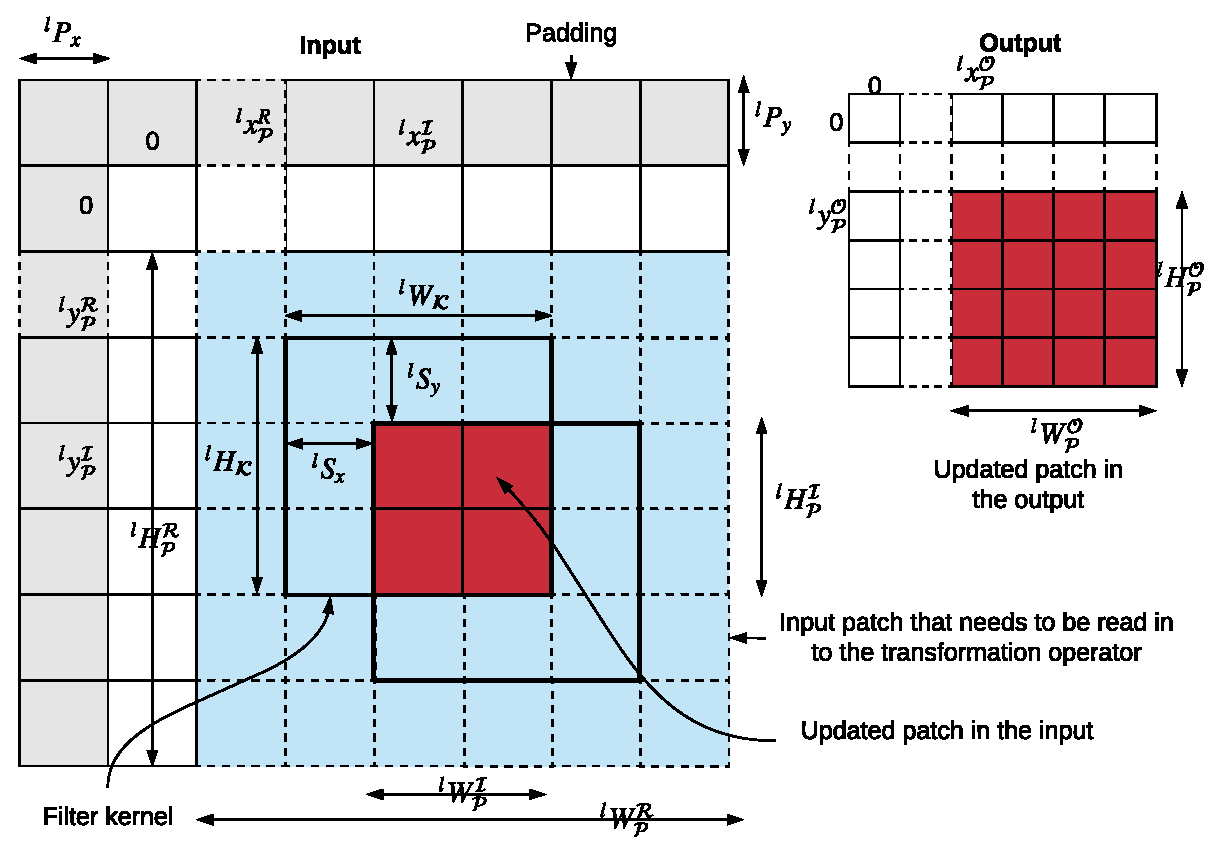
\includegraphics[width=\columnwidth]{images/dimensions}
\vspace{-8mm}
\caption{Simplified illustration of input and output update patches for Convolution/Pooling layers.}
\label{fig:dimensions}
\end{figure}


Equation~(\ref{eqn:xcoordinate}) calculates the coordinates of the output update patch. Padding effectively shifts the coordinate system and thus, $P_{x:l}$ is added to correct it. Due to overlaps among the filter kernels, the affected region of the input update patch will be increased by $W_{\mathcal{K}:l}-1$, which needs to be subtracted from the input coordinate $x^\mathcal{I}_{\mathcal{P}:l}$. A filter of size $W_{\mathcal{K}:l}$ that is placed starting at $x^\mathcal{I}_{\mathcal{P}:l} - W_{\mathcal{K}:l} + 1$ will see an update starting from $x^\mathcal{I}_{\mathcal{P}:l}$. Equation~(\ref{eqn:patchwidth}) calculates the width of the output update patch. Given these, a start coordinate and width of the read-in context are given by Equations~(\ref{eqn:xreadcoordinate}) and~(\ref{eqn:readpatchwidth}); similar equations hold for the height dimension (skipped for brevity).


\begin{table}[t]
  \centering
  \scalebox{0.8}{\begin{tabular}{p{2cm}p{7.5cm}}
    \toprule
    \textbf{Symbol} & \textbf{Meaning}\\
    \midrule \midrule
    $x^\mathcal{I}_{\mathcal{P}:l}, y^\mathcal{I}_{\mathcal{P}:l}$ & Starting coordinates of the input patch for the $l^{th}$ layer\\
    \midrule
    $x^\mathcal{R}_{\mathcal{P}:l}, y^\mathcal{R}_{\mathcal{P}:l}$ & Starting coordinates of the patch that needs to be read in for the $l^{th}$ layer transformation\\
    \midrule
    $x^\mathcal{O}_{\mathcal{P}:l}, y^\mathcal{O}_{\mathcal{P}:l}$ & Starting coordinates of the output patch for the $l^{th}$ layer\\
    \midrule
    $H^\mathcal{I}_{\mathcal{P}:l}, W^\mathcal{I}_{\mathcal{P}:l}$ & Height and width of the input patch for the $l^{th}$ layer\\
   	\midrule
   	$H^\mathcal{R}_{\mathcal{P}:l}, W^\mathcal{R}_{\mathcal{P}:l}$ & Height and width of the patch that needs to be read in for the $l^{th}$ layer transformation\\
   	\midrule
   	$H^\mathcal{O}_{\mathcal{P}:l}, W^\mathcal{O}_{\mathcal{P}:l}$ & Height and width of the output patch for the $l^{th}$ layer\\
    \midrule
    $\tau$ & Projective field threshold\\
    \midrule
    $r_{drill-down}$ & Stage two drill-down fraction used in \textit{adaptive drill-down}\\
    \bottomrule
  \end{tabular}}
\caption{Additional notation for Sections~\ref{sec:exact} and~\ref{sec:approx}.}
\label{table:optimizer_symbols}
\end{table}

\vspace{2mm}
\noindent \textbf{Incremental Inference Operation.}
For layer $l$, given the transformation function $T_{:l}$, the pre-materialized input tensor $\mathcal{I}_{:l}$, input update patch $\mathcal{P}^\mathcal{O}_{:l}$, and the above calculated coordinates and dimensions of the input, output, and read-in context, the output update patch $\mathcal{P}^\mathcal{O}_{:l}$ is computed as follows:

\begin{align}
\label{eqn:readin}
\mathcal{U} =&~ \mathcal{I}_{:l}[:,x^\mathcal{R}_{\mathcal{P}:l}:x^\mathcal{R}_{\mathcal{P}:l}+W^\mathcal{R}_{\mathcal{P}:l}, y^\mathcal{R}_{\mathcal{P}:l}: y^\mathcal{R}_{\mathcal{P}:l}+ H^\mathcal{R}_{\mathcal{P}:l}]\\
\label{eqn:superposition}
\mathcal{U} =&~ \mathcal{U} \bm\circ_{(x^\mathcal{I}_{\mathcal{P}:l}-x^\mathcal{R}_{\mathcal{P}:l}),(y^\mathcal{I}_{\mathcal{P}:l}-y^\mathcal{R}_{\mathcal{P}:l})} \mathcal{P}^{\mathcal{I}}_{:l}\\
\label{eqn:callt}
\mathcal{P}^\mathcal{O}_{:l} =&~ T_{:l}(\mathcal{U})
\end{align}

Equation~(\ref{eqn:readin}) slices the read-in context $\mathcal{U}$ from the pre-materialized input tensor $\mathcal{I}_{:l}$. Equation~(\ref{eqn:superposition}) superimposes the input update patch $\mathcal{P}^\mathcal{I}_{:l}$ on it. This is an in-place update of the array holding the read-in context. Finally, Equation~(\ref{eqn:callt}) computes the output update patch $\mathcal{P}^{\mathcal{O}}_{:l}$ by invoking $T_{:l}$ on $\mathcal{U}$. Thus, we avoid performing inference on all of $\mathcal{I}_{:l}$, thus achieving incremental inference and reducing FLOPs.


\subsection{Propagating Updates across Layers}

\vspace{2mm}
\noindent \textbf{Sequential CNNs.} Unlike relational IVM, CNNs consist of many layers, often in a sequence. This is analogous to having not just one query, but a sequence of queries that require IVM on their predecessor's updated output. This leads to a new issue--correctly and automatically configuring the update patches across all layers of a CNN. Specifically, output update patch $\mathcal{P}^{\mathcal{O}}_{:l}$ of layer $l$ becomes the input update patch of layer $l+1$. While this seems simple, it requires care at the boundary of a local context transformation and a global context transformation, e.g., going from a Convolution layer (or Pooling layer) to a Fully-Connected layer. In particular, we need to materialize the \textit{full updated output} instead of propagating just the output update patches, since the global context transformation might lose spatial locality for subsequent layers.

\vspace{2mm}
\noindent \textbf{Extension to DAG CNNs.} Some recent deep CNNs have their layers organized as a more general directed acyclic graph (DAG) instead of a sequence. Such CNNs contain two additional layers apart from the layers described earlier: \textit{element-wise addition} and \textit{depth-wise concatenation}, which are needed to ``merge'' two branches in the DAG. Element-wise addition requires two input tensors with all dimensions being identical. Depth-wise concatenation takes two input tensors with the same height and width dimensions. We now face a new challenge--how to calculate the output update patch when the two input tensors differ on their input update patches locations and sizes? Figure~\ref{fig:la_operators} shows a simplified illustration of this issue. The first input has its update patch starting at coordinates $(x^\mathcal{I}_{\mathcal{P}_1:l},y^\mathcal{I}_{\mathcal{P}_1:l})$ with dimensions $H^\mathcal{I}_{\mathcal{P}_1:l}$ and $W^\mathcal{I}_{\mathcal{P}_1:l}$, while the second input has its update patch starting at coordinates $(x^\mathcal{I}_{\mathcal{P}_2:l},y^\mathcal{I}_{\mathcal{P}_2:l})$ with dimensions $H^\mathcal{I}_{\mathcal{P}_2:l}$ and $W^\mathcal{I}_{\mathcal{P}_2:l}$. This issue can arise with both element-wise addition and depth-wise concatenation. 

\begin{figure}[t]
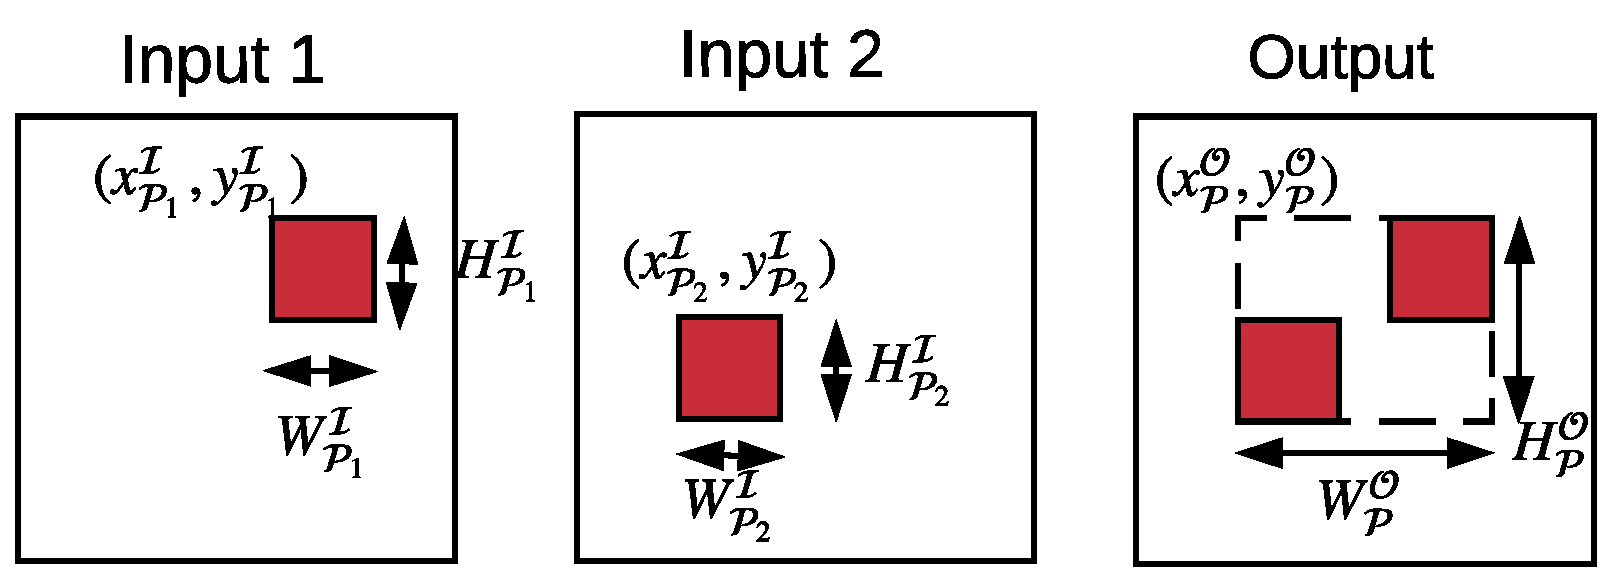
\includegraphics[width=\columnwidth]{images/la_operators}
\vspace{-8mm}
\caption{Illustration of bounding box calculation for differing input update patch locations for element-wise addition and depth-wise concatenation layers in DAG CNNs.}
\label{fig:la_operators}
\end{figure}

We propose a simple unified solution: compute the \textit{bounding box} of both the input update patches. This means the coordinates and dimensions of both the output update patch and both the read-in contexts will be identical. Figure~\ref{fig:la_operators} illustrates this too. While our solution will potentially recompute portions of the output that did not get modified, we think this trade-off is acceptable because the gains are likely to be marginal for the additional complexity introduced into our framework. Overall, the output update patch coordinate and width dimension are given by the following (similarly for the height dimension):

\vspace{-4mm}
\begin{align}
\begin{split}
x^\mathcal{O}_{P:l} =&~ \texttt{min}(x^\mathcal{I}_{\mathcal{P}_1:l}, x^\mathcal{I}_{\mathcal{P}_2:l})\\
% y^\mathcal{O}_\mathcal{P} = y^\mathcal{R}_\mathcal{P} =&~ \texttt{min}(y^\mathcal{I}_{\mathcal{P}_1},y^\mathcal{I}_{\mathcal{P}_2})\\
% \label{eqn:lapatchwidth}
W^\mathcal{O}_{\mathcal{P}:l} =&~ \texttt{max}(x^\mathcal{I}_{\mathcal{P}_1:l}+W^\mathcal{I}_{\mathcal{P}_1:l},x^\mathcal{I}_{\mathcal{P}_2:l}+W^\mathcal{I}_{\mathcal{P}_2:l}) -\texttt{min}(x^\mathcal{I}_{\mathcal{P}_1:l},x^\mathcal{I}_{\mathcal{P}_2:l})
% H^\mathcal{O}_\mathcal{P} = H^\mathcal{R}_\mathcal{P} =&~ \texttt{max}(y^\mathcal{I}_{\mathcal{P}_1}+H^\mathcal{I}_{\mathcal{P}_1},y^\mathcal{I}_{\mathcal{P}_2}+H^\mathcal{I}_{\mathcal{P}_2})-\texttt{min}(y^\mathcal{I}_{\mathcal{P}_1},y^\mathcal{I}_{\mathcal{P}_2})
\end{split}
\end{align}

\subsection{Multi-Query Incremental Inference}
As explained in Section~\ref{sec:problem}, the OBE workload issues multiple ($|G|$ to be precise) re-inference requests \textit{in one go} for different occlusion patch locations.
Viewig each re-inference request as a ``query'' itself, we now make a connection with multi-query optimization (MQO)~\cite{sellis}.
We observe that the $|G|$ queries are \textit{not disjoint}--they share large parts of the input, since the occlusion patch is typically much smaller than the image.
Thus, we now extend our incremental inference optimization and integrate it with an MQO-style optimization for OBE.
To the best of our knowledge, this is the first known instance of fusing an IVM-style techniques with an MQO-style technique for optimizing CNN inference.
To draw an analogy to relational optimization, this situation is like a batch of incremental update queries arriving at once on the same relation, with each query modifying a different but small part of the input relation.

\vspace{2mm}
\noindent \textbf{Batched Incremental Inference.}
Our optimization works as follows: materialize all the tensors produced by the CNN's layers \textit{once}. Then, \textit{reuse} these tensors for incremental inference for each of the $|G|$ queries. This is feasible due to our above observation--most of the occluded image's pixels are still identical across the queries, which means large parts of the tensors produced by a given CNN layer will likely be identical too. Essentially, we amortize the cost of materializing the tensors across all $|G|$ queries.
%We also apply system specific optimizations to improve performance in the high throughput GPU environment.
One might wonder, why not just perform ``batched'' inference for the $|G|$ queries? Batched inference is standard practice today for high-throughput compute hardware such as GPUs, since it amortizes the CNN set up costs, data movement costs, etc. Batch sizes are picked to optimize hardware utilization.
Our answer is that batched inference is an \textit{orthogonal} (albeit trivial) optimization compared to our above optimization.
In other words, we can combine these two ideas and execute incremental inference in a batched manner. We call this approach ``batched incremental inference.''
As we show later (Section 5), batching alone yields only modest 2X speedups, while combining batching and incremental inference amplifies the speedups.
Algorithm~\ref{alg:incinference} formally presents the batched incremental inference operation for layer $l$.

\begin{algorithm}
    \caption{\textproc{BatchedIncrementalInference}}
    \label{alg:incinference}
    \begin{flushleft}
     \hspace*{1mm} \textbf{Input:} \\
     \hspace*{3mm} $T_{:l}$ : \textit{Original Transformation function}\\
     \hspace*{3mm} $\mathcal{I}_{:l}$ : \textit{Pre-materialized input from original image}\\
     \hspace*{3mm} $[\mathcal{P^I}_{1:l},...,\mathcal{P^I}_{n:l}]$ : \textit{Input patches}\\
     \hspace*{3mm} $[(x^\mathcal{I}_{\mathcal{P}_1:l},y^\mathcal{I}_{\mathcal{P}_1:l}),...,(x^\mathcal{I}_{\mathcal{P}_n:l},y^\mathcal{I}_{\mathcal{P}_n:l})]$ : \textit{Input patch coordinates}\\
     \hspace*{3mm} $W^\mathcal{I}_{\mathcal{P}:l},H^\mathcal{I}_{\mathcal{P}:l}$ : \textit{Input patch dimensions}
    \end{flushleft}

\eat{    \begin{flushleft}
     \hspace*{1mm} \textbf{Output:}\\
     \hspace*{3mm} $[\mathcal{P^O}_{1:l},...,\mathcal{P^O}_{n:l}]$ : \textit{Output patches}\\
     \hspace*{3mm} $[(x^\mathcal{O}_{\mathcal{P}_1:l},y^\mathcal{O}_{\mathcal{P}_1:l}),...,(x^\mathcal{O}_{\mathcal{P}_n:l},y^\mathcal{O}_{\mathcal{P}_n:l})]$ : \textit{Output patch coordinates}\\
     \hspace*{3mm} $W^\mathcal{O}_{\mathcal{P}:l},H^\mathcal{O}_{\mathcal{P}:l}$ : \textit{Output patch dimensions}
    \end{flushleft}}

    \begin{algorithmic}[1]
    \Procedure{BatchedIncrementalInference}{}
    \State \textit{Calculate} $[(x^\mathcal{O}_{\mathcal{P}_1:l},y^\mathcal{O}_{\mathcal{P}_1:l}),...,(x^\mathcal{O}_{\mathcal{P}_n:l},y^\mathcal{O}_{\mathcal{P}_n:l})]$ 
    \State \textit{Calculate} ($W^\mathcal{O}_{\mathcal{P}:1},H^\mathcal{O}_{\mathcal{P}:l}$)
    \State \textit{Calculate} $[(x^\mathcal{R}_{\mathcal{P}_1:l},y^\mathcal{R}_{\mathcal{P}_1:l}),...,(x^\mathcal{R}_{\mathcal{P}_n:l},y^\mathcal{R}_{\mathcal{P}_n}:l)]$
    \State \textit{Calculate} ($W^\mathcal{R}_{\mathcal{P}:l},H^\mathcal{R}_{\mathcal{P}:l}$)
    \State \textit{Initialize} $\mathcal{U} \in \mathcal{\rm I\!R}^{n \times \texttt{depth}(\mathcal{I}_{:l}) \times H^\mathcal{R}_{\mathcal{P}:l} \times W^\mathcal{R}_{\mathcal{P}:l}}$

    \For{\texttt{i in [1,...,n]}}\label{alg:line:memcpy_loop}
        \State $T_1 \gets \mathcal{I}_{:l}[:,x^\mathcal{R}_{\mathcal{P}_i:l}:x^\mathcal{R}_{\mathcal{P}_i:l}+W^\mathcal{R}_{\mathcal{P}:l},y^\mathcal{R}_{\mathcal{P}_i:l}:y^\mathcal{R}_{\mathcal{P}_i:l}+H^\mathcal{R}_{\mathcal{P}:l}]$ 
        \State $T_2 \gets T_1 \bm\circ_{(x^\mathcal{I}_{\mathcal{P}_i:l}-x^\mathcal{R}_{\mathcal{P}_i:l}),(y^\mathcal{I}_{\mathcal{P}_i:l}-y^\mathcal{R}_{\mathcal{P}_i:l})} \mathcal{P}_{i:l}$
        \State $\mathcal{U}[i,:,:] \gets T_2$
    \EndFor

    \State $[\mathcal{P}^\mathcal{O}_{1:l},...,\mathcal{P}^\mathcal{O}_{n:l}] \gets T(\mathcal{U})$ \Comment{Batched version}
    \State \textbf{return} $[\mathcal{P}^\mathcal{O}_{1:l},...,\mathcal{P}^\mathcal{O}_{n:l}]$,
    \State \hspace*{5mm} $[(x^\mathcal{O}_{\mathcal{P}_1:l},y^\mathcal{O}_{\mathcal{P}_1:l}),...,(x^\mathcal{O}_{\mathcal{P}_n:l},y^\mathcal{O}_{\mathcal{P}_n:l})],$ ($W^\mathcal{O}_{\mathcal{P}:l},H^\mathcal{O}_{\mathcal{P}:l}$) 
    \EndProcedure
    \end{algorithmic}

% \eat{%Maybe in the Appendix
%     \vspace*{-2mm}
%     \hrulefill
    
%     \begin{flushleft}
%      \hspace*{4mm} \textbf{Input:}\\
%      \hspace*{8mm} $\mathcal{O}$ : \textit{Pre-materialized output from original image}\\
%      \hspace*{8mm} $[\mathcal{P}^\mathcal{O}_1,...,\mathcal{P}^\mathcal{O}_n]$ : \textit{Output patches}\\
%      \hspace*{8mm} $[(x^\mathcal{O}_{\mathcal{P}_1},y^\mathcal{O}_{\mathcal{P}_1}),...,(x^\mathcal{O}_{\mathcal{P}_n},y^\mathcal{O}_{\mathcal{P}_n})]$ : \textit{Output patch coordinates}\\
%     \end{flushleft}

%     \begin{flushleft}
%      \hspace*{4mm} \textbf{Output:}\\
%      \hspace*{8mm} $O\textrm'$ : \textit{Updated output}
%     \end{flushleft}
%   \begin{algorithmic}[1]
%     \Procedure{IncrementalToFullProjection}{}
%     \State \textit{Initialize} $\mathcal{O}\textrm' \in \mathcal{\rm I\!R}^{n \times \texttt{depth}(\mathcal{O}) \times \texttt{height}(\mathcal{O}) \times \texttt{width}(\mathcal{O})}$
%     \For{\texttt{i in [1,...,n]}}
%       \State $T \gets \texttt{copy}(O)$
%       \State $\mathcal{O}\textrm'[i,:,:] \gets T \bm\circ_{x^\mathcal{O}_{\mathcal{P}_i},y^\mathcal{O}_{\mathcal{P}_i}} \mathcal{P}^\mathcal{O}_i$
%     \EndFor
%     \State \textbf{return} $\mathcal{O}\textrm'$
%     \EndProcedure
%     \end{algorithmic}
% }
\end{algorithm}


\eat{
The \textproc{BatchedIncrementalInference} procedure takes in the original transformation of the layer, pre-materialized input for the layer corresponding to the original image, a batch of updated patches which are 3D volumes of activation values and their geometric properties as input.
}

\textproc{BatchedIncrementalInference} first calculates the geometric properties of the output update patches and read-in contexts. A temporary tensor $U$ is initialized to hold the input update patches with their read-in contexts. The \textbf{for} loop iteratively populates $U$ with corresponding patches. Finally, $T_{:l}$ is applied to $U$ to compute the output patches. We note that only for the first layer, all input update patches will be identical to the occlusion patch. But for the later layers, the update patches will start to deviate depending on their locations and read-in contexts.


\vspace{2mm}
\noindent \textbf{GPU Optimized Implementation.}
Empirically, we observed an interesting dichotomy between CPUs and GPUs: \textproc{BatchedIncrementalInference} yields expected speedups on CPUs, but it performs dramatically poorly on GPUs. Indeed, a naive implementation of \textproc{BatchedIncrementalInference} on GPUs was often \textit{slower} than full inference! We now explain why this is the case and how we tackled this issue. The \textbf{for} loop in line~\ref{alg:line:memcpy_loop} of Algorithm~\ref{alg:incinference} is essentially preparing the input for $T_{:l}$ by copying values (slices of the materialized input tensor) from one part of the GPU memory to another \textit{sequentially}. A detailed profiling of the GPU showed that such sequential memory copies are a bottleneck for the naive GPU implementation, since the GPU is throttled from exploiting its massive parallelism effectively. To overcome this GPU-specific issue, we created a custom CUDA kernel to perform the input preparation more efficiently by copying the memory regions in parallel for all items in the batched inference request. Essentially, this is a parallel \textbf{for} loop customized for slicing the input tensor. We then invoke the CNN transformation function $T_{:l}$, which is already highly hardware-optimized by modern deep learning tools~\cite{chetlur2014cudnn}. We defer more details on our custom CUDA kernel to the appendix due to space constraints. Also, since GPU memory might not be enough to fit all $|G|$ queries, the batch size for the GPU-based execution might be smaller than $|G|$. Overall, our incremental inference optimizations yield benefits directly in the CPU environment but requires our custom kernel for the GPU environment.
%\red{TODO: Refer to hardware works, e.g. Li Tseng, Lin, Swanson, Yannis on hardware accelerators}


\subsection{Putting it All Together}

We now summarize the end-to-end workflow of our incremental inference optimizations for the OBE workload.
We are given the CNN $f$, image $\mathcal{I}_{:img}$, predicted class label $L$, occlusion patch $\mathcal{P}$ and its stride $S_{\mathcal{P}}$, and the set of occlusion patch positions $G$.
Pre-materialize the output tensors of all layers of $f$ with $\mathcal{I}_{:img}$ as the input.
Prepare the occluded images ($\mathcal{I}^{'}_{(x,y):img}$) for all positions in $G$.
For batches of $\mathcal{I}^{'}_{(x,y):img}$ as the input, invoke the transformations in $f$ in topological order and calculate the corresponding entries of the heat map $M$.
For local context transformations, invoke \textproc{BatchedIncrementalInference}.
For a local context transformation that precedes a global context transformation, materialize the full updated output.
For all other layers, invoke the original transformation function.
$M$ is now the output heat map.


\section{Approximate Inference Optimizations}\label{sec:approx}
In this Section, we explain \textit{projective field thresholding} and \textit{adaptive drill-down}, which are two \textit{approximate inference} optimizations used in ~\system.
We also explain how \system~ tunes its internal system configuration parameters for these \textit{approximate inference} optimizations.


\subsection{Projective Field Thresholding}
Projective field \cite{le2017receptive, basiccnnoperations} of a CNN neuron is the local region (including the depth) of the output 3-D tensor which is connected to it.
The term is borrowed from the Neuroscience field where it is used to describe the spatiotemporal effects exerted by a retinal cell on all of the outputs of the neuronal circuitry \cite{de2011projective}.
For our work, the notion of projective field is useful as it determines the change propagation path for incremental changes.
The three types of CNN transformations affect the size of the projective field differently.
Point transformations do not change the projective field size while global context transformations increase it to the maximum.
Transformations that operate on a local spatial context increase it gradually.
The amount of increase in a local context transformation is determined by the filter size and stride parameters.
At every transformation, the size of the projective field will increase linearly by the filter size and multiplicatively by the stride value.

\begin{figure}[t]
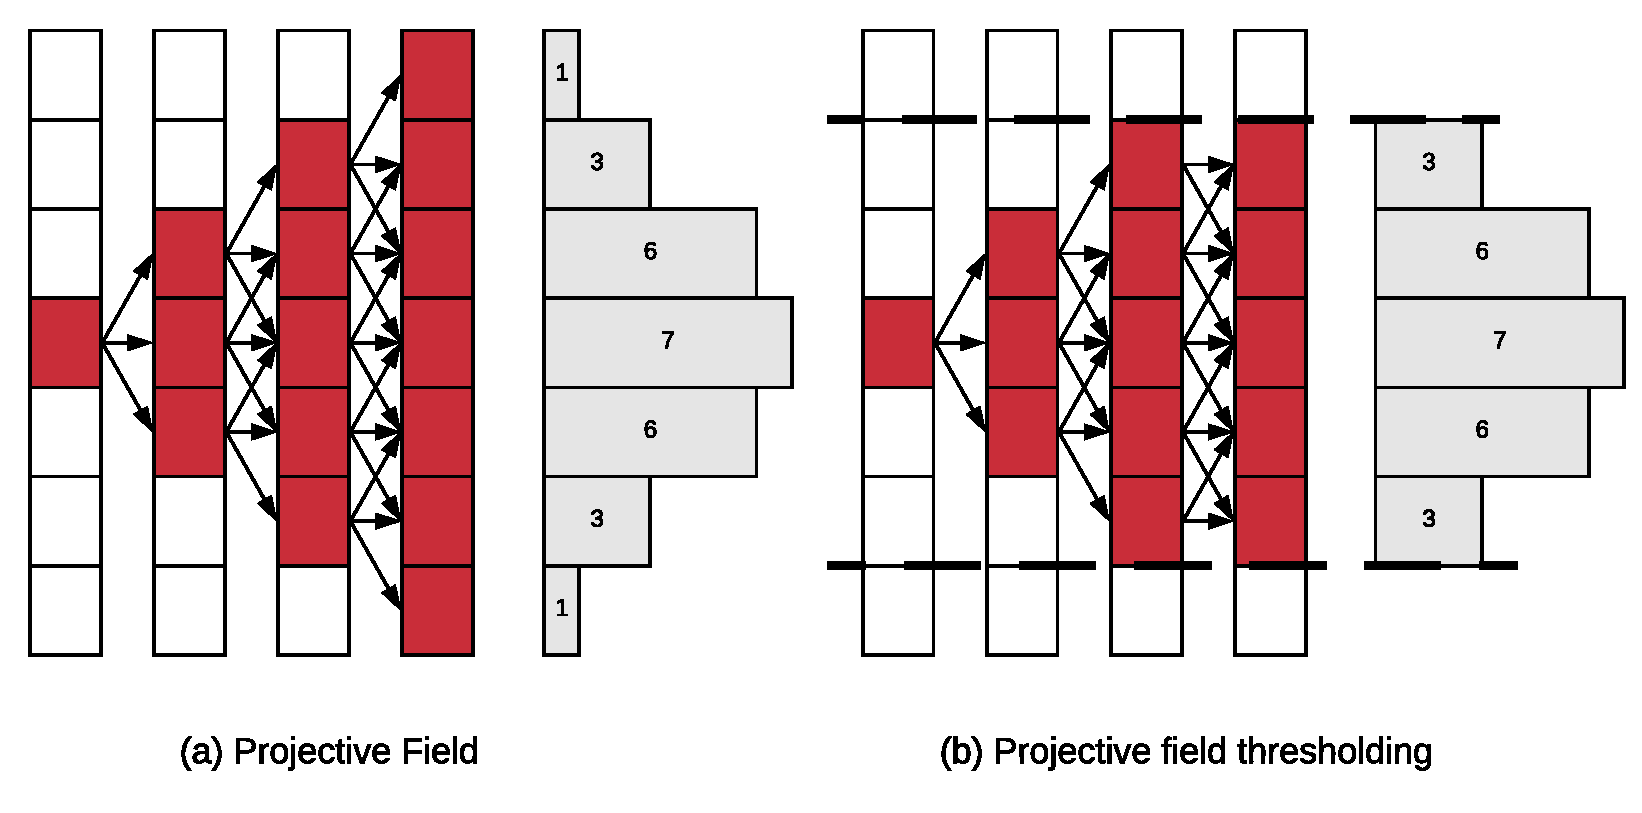
\includegraphics[width=\columnwidth]{images/pf_truncate}
\caption{(a) One dimensional Convolution demonstrating projective field growth (filter size = 2, stride = 1). (b) \textit{Projective field thresholding} with $\tau = 5/7$.}
\label{fig:pf_truncate}
\end{figure}

Because of the projective field growth, even though there will be many computational redundancies in the early layers, towards the latter layers it will decrease or even have no redundancies.
However, we empirically found that the projective field growth can be restrained up to a certain extent without significantly sacrificing the accuracy.
For a more intuitive understanding of why this would work consider the simplified 1-D Convolution example shown in Figure \ref{fig:pf_truncate} (a).
In the example, a single neuron is modified (marked in red) and a filter of size three is applied with a stride of one repeatedly four times.
Since the filter size is three, each updated neuron will propagate the change to three neurons in the next output layer causing the projective field to grow linearly.
The histogram at the end of the fourth layer shows the number of unique paths that are available between each output neuron and the originally updated neuron in the first layer.
It can be seen that this distribution resembles a Gaussian where many of the paths are connected to the central region.
The amount of change in the output layer is determined by both the number of unique paths and also the individual weights of the connections.
It can be shown that the distribution of change in the output layer will converge to a Gaussian distribution provided certain conditions are met for the weight values of the filter kernel (more details in Appendix X).
\eat{
For more details we refer the reader to \cite{luo2016understanding}, where a similar theoretical result has been proved for the receptive field\footnote{Receptive field of a CNN neuron is the local region (including the depth) of the input volume which is connected to it.} of a Deep CNN.
}

As most of the change will be concentrated on the center we introduce the notion of a projective field threshold $\tau ~ (0 < \tau \leq 1)$ which will be used to restrict the growth of the projective field.
It determines the maximum size of the projective field as a fraction of the size of the output.
Figure \ref{fig:pf_truncate} (b) demonstrates the application of projective field thresholding with a $\tau$ value of $5/7$.
From the histogram generated for the projective field thresholding approach, we can expect that much of the final output change is maintained by this approach.

In \system, \textit{projective field thresholding} is implemented on top of \textit{incremental inference} approach by applying set of additional constraints on input-output coordinate mappings. For the horizontal dimension (similarly for vertical dimension) the new set of calculations can be expressed as follows:

\begin{align}
\label{eqn:normal_width_calc}
W^\mathcal{O}_{\mathcal{P}:l} = &~ \texttt{min}\big(\lceil (W^\mathcal{I}_{\mathcal{P}:l} + W_{\mathcal{K}:l} - 1)/S_{x:l} \rceil, W^\mathcal{O}_{\mathcal{P}:l}\big)\\
\label{eqn:check_tau}
\text{If}~ W_{\mathcal{P}:l}^\mathcal{O} & > \texttt{round}(\tau \times W^\mathcal{O}_{:l}):\\
\label{eqn:new_width_calc_with_tau}
& W^\mathcal{O}_{\mathcal{P}:l} = \texttt{round}(\tau \times W^\mathcal{O}_{:l})\\
\label{eqn:new_in_width}
& W^\mathcal{I}_{\mathcal{P}_{new}:l} = W^\mathcal{O}_{\mathcal{P}:l} \times S_{x:l} - W_{\mathcal{K}:l} + 1\\
\label{eqn:new_x_coord}
& x^{\mathcal{I}}_{\mathcal{P}:l} \mathrel{+}= (W^\mathcal{I}_{\mathcal{P}:l} - W^\mathcal{I}_{\mathcal{P}_{new}:l})/2\\
\label{eqn:new_input_width}
& W^\mathcal{I}_{\mathcal{P}:l} = W^\mathcal{I}_{\mathcal{P}_{new}:l}\\
\label{eqn:new_output_x}
x^\mathcal{O}_{\mathcal{P}:l} = & \texttt{max}\big(\lceil (P_{x:l} + x^\mathcal{I}_{\mathcal{P}:l} - W_{\mathcal{K}:l} + 1)/S_{x:l} \rceil, 0\big)
\end{align}

Equation (\ref{eqn:normal_width_calc}) calculates output width assuming no thresholding.
But if the output width exceeds the threshold defined by $\tau$, output width is set to the threshold value as per Equation (\ref{eqn:new_width_calc_with_tau}).
Equation \ref{eqn:new_in_width} calculates the input width that would produce an output of width $W^\mathcal{O}_{\mathcal{P}:l}$ (think of this as making $W^{\mathcal{I}}_{\mathcal{P}:l}$ the subject of equation \ref{eqn:normal_width_calc}).
If the new input width is smaller than the original input width, the starting x coordinate should be updated as per Equation (\ref{eqn:new_x_coord}) such that the updated coordinates correspond to a center crop from the original.
Equation (\ref{eqn:new_input_width}) set the input width to the newly calculated input width and Equation (\ref{eqn:new_output_x}) calculates the x coordinate of the output patch from the updated values.

\begin{figure}[t]
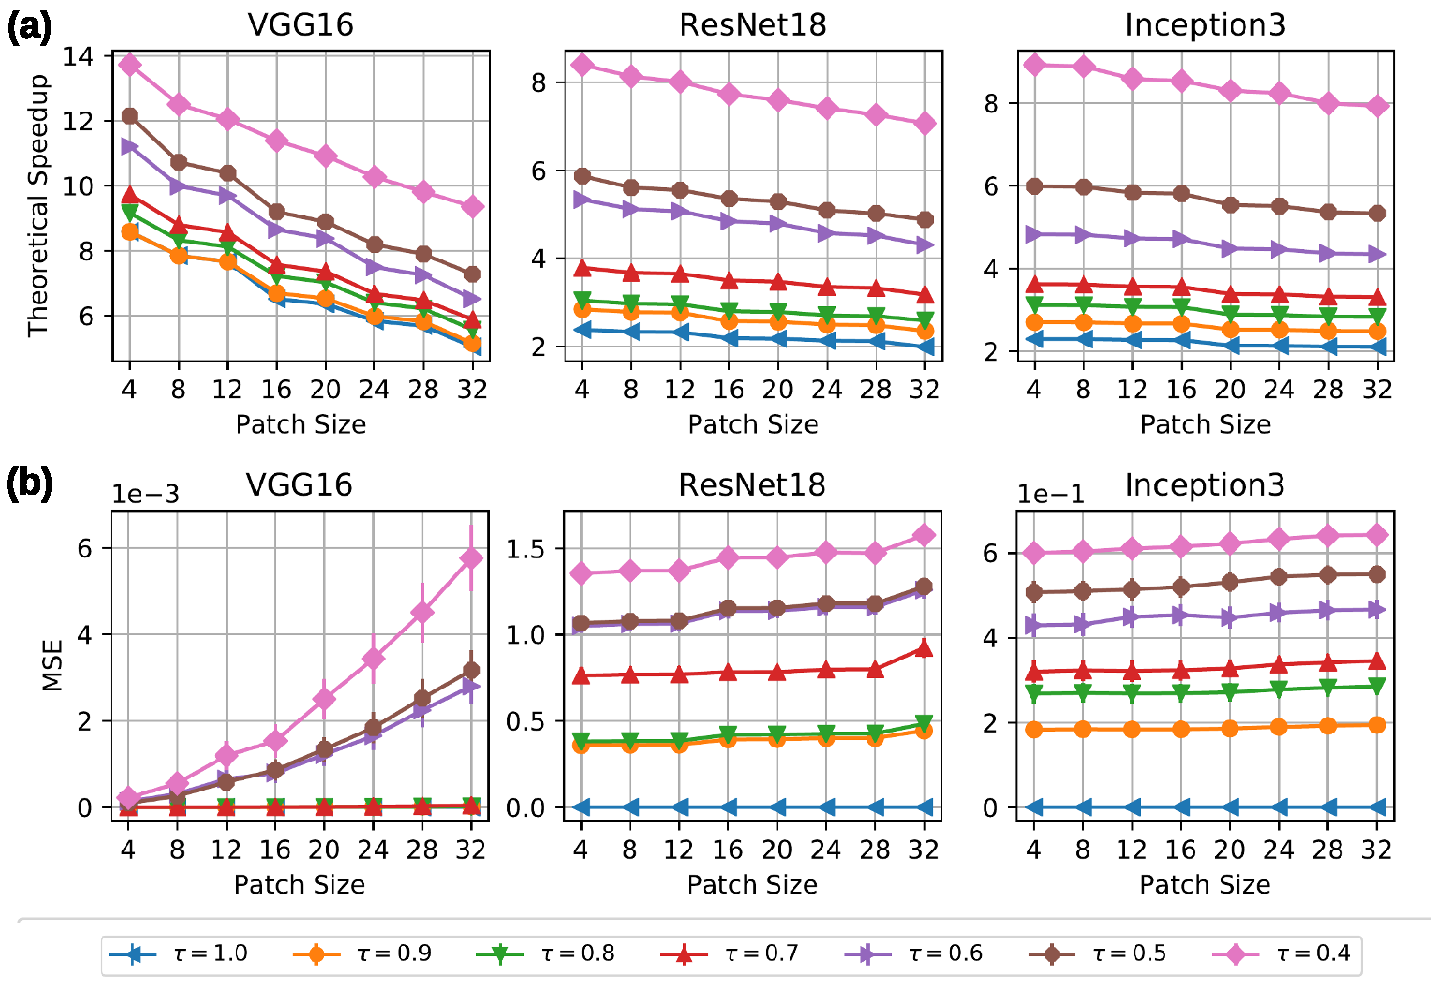
\includegraphics[width=\columnwidth]{images/proj_thresholding}
\caption{(a) Theoretical speedup ratio with projective field thresholding. (b) Mean Square Error between exact and approximate output of the final Convolution or Pool transformation.}
\label{fig:proj_thresholding}
\end{figure}

\vspace{2mm}
\noindent \textbf{Theoretical Speedup with Projective Field Thresholding.}
We analyze the theoretical speedup that can be achieved with \textit{projective field thresholding} approach when a square occlusion patch is placed on the center of the input image.
Figure \ref{fig:proj_thresholding} (a) presents the results.
It can be seen that with increasing $\tau$ attainable theoretical speedup also increases.
We also analyze the mean square error (MSE) between the exact and approximate output tensors produced by the final Convolution or Pool transformation with a black occlusion patch placed on the center of the input image.
The results are shown in Figure \ref{fig:proj_thresholding} (b).
With increasing $\tau$ and increasing patch size we see that the MSE is also increasing.


\subsection{Adaptive Drill-Down}\label{sec:ada-drill-down}
\textit{Adaptive drill-down} approach, which is only applicable in the non-interactive mode, is based on the observation that in many occlusion based explainability workloads, such as in medical imaging, the regions of interest will occupy only a small fraction of the entire image.
In such cases, it is unnecessary to inspect the entire image at a higher resolution with a small stride value for the occlusion patch.
In \textit{adaptive-drill-down} the final occlusion heat map will be generated using a two-stage process.
At the first stage, a low-resolution heat map will be generated by using a larger stride which we call stage one stride $S_1$.
From the heat map generated at stage one, a predefined drill-down fraction $r_{drill-down}$ of regions with highest probability drop for the predicted class is identified.
At stage two a high-resolution occlusion map is generated using the original user provided stride value, also called stage two stride $S_2$, only for the selected region.
A schematic representation of \textit{adaptive drill-down} is shown in Figure \ref{fig:adaptive_drill_down} (a).

% \begin{figure}[t]
% 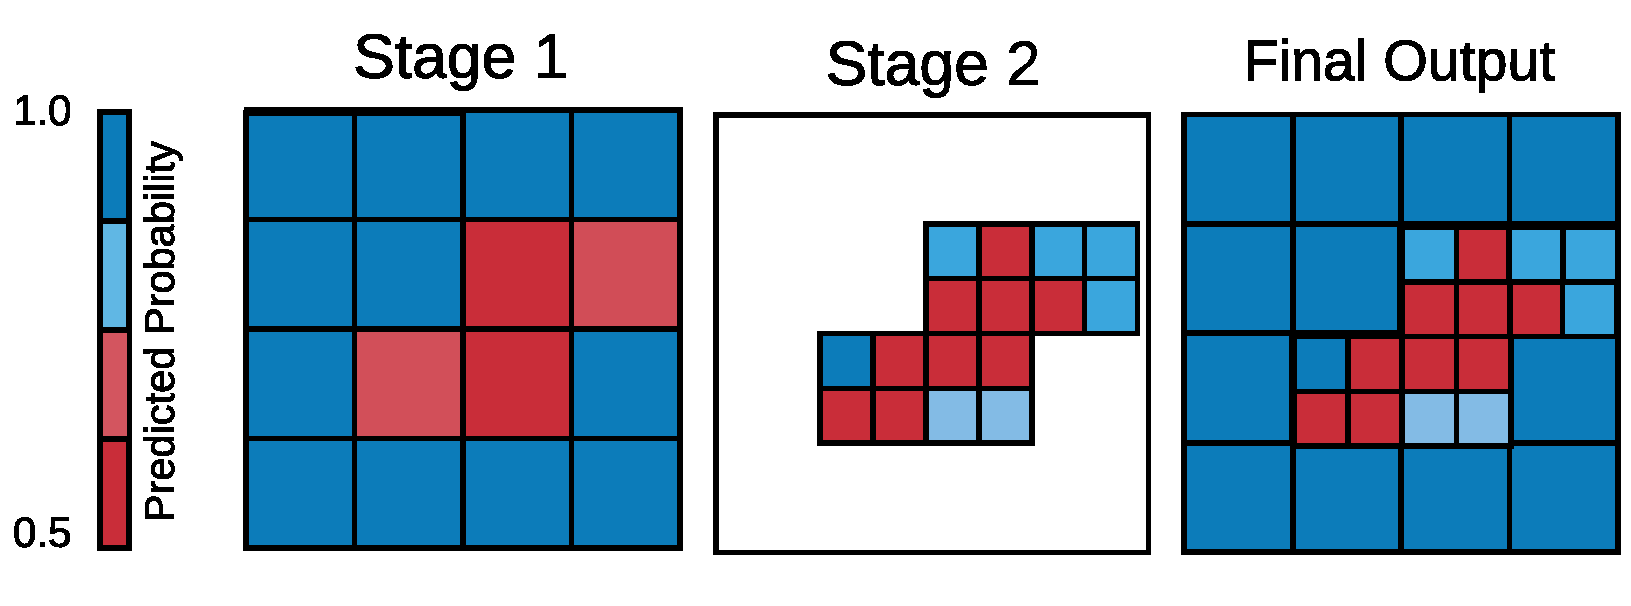
\includegraphics[width=\columnwidth]{images/adaptive-drill-down}
% \caption{Schematic representation of \textit{adaptive drill-down}}
% \label{fig:adaptive-drill-down}
% \end{figure}

The amount of speedup that can be obtained from \textit{adaptive drill-down} is determined by both $r_{drill-down}$ and $S_1$.
If the $r_{drill-down}$ is low, only a small region will have to be examined at a higher resolution and thus it will be faster.
However, this smaller region may not be sufficient to cover all the interesting regions on the image and hence can result in losing important information.
Larger $S_1$ also reduces the overall runtime as it reduces the time taken for stage one.
But it has the risk of misidentifying interesting regions especially when the granularity of those regions are smaller than the occlusion patch size.
The speedup obtained by \textit{adaptive drill-down} approach is equal to the ratio between the number of individual occlusion patch positions generated for the normal and \textit{adaptive drill-down} approaches.
Number of individual occlusion patch positions generated with a stride value of $S$ is proportional to $1/S^2$ (total number of patch positions is equal to $\frac{H_{\mathcal{I}_{img}}}{S} \times \frac{W_{\mathcal{I}_{img}}}{S}$).
Hence the speedup can  be expressed as per Equation \ref{eqn:adaptive-drill-down-eqn}.
Figure \ref{fig:adaptive_drill_down} (b) conceptually shows how the speedup would vary with $S_1$ when $r_{drill-down}$ is fixed and vice versa.

\begin{align}
\label{eqn:adaptive-drill-down-eqn}
\texttt{speedup} = \frac{S^2_1}{S^2_2+r_{drill-down} \times S^2_1}
\end{align}

\begin{figure}[t]
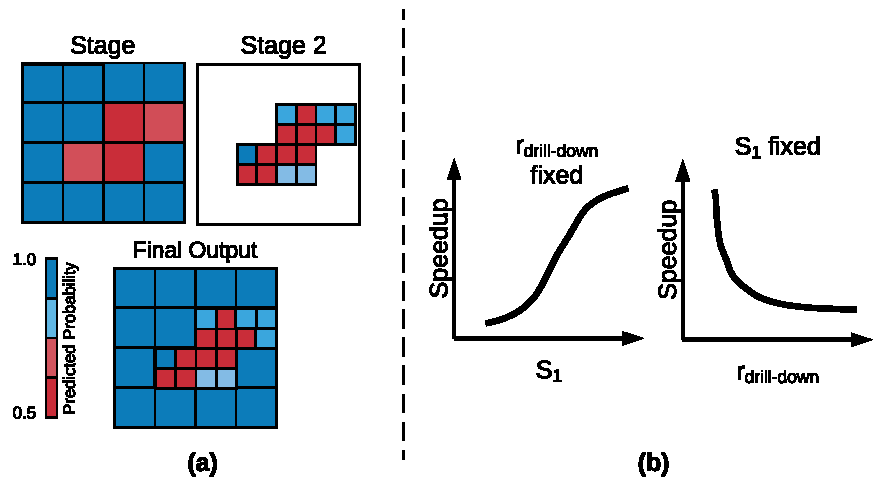
\includegraphics[width=\columnwidth]{images/adaptive_drill_down}
\caption{(a) Schematic representation of \textit{adaptive drill-down}. (b) Conceptual diagram showing the effect of $S_1$ and $r_{drill-down}$ on speedup. }
\label{fig:adaptive_drill_down}
\end{figure}

\subsection{System Tuning}
In this section we explain how \system~ sets its internal configuration parameters for \textit{approximate inference} optimizations.

\vspace{2mm}
\noindent \textbf{Tuning projective field threshold.}
The inaccuracies incurred when applying \textit{projective field thresholding} can cause quality degradation in the generate approximate heat map all the way from indistinguishable changes major structural changes.
To measure this quality degradation we use Structural Similarity (SSIM) Index~\cite{wang2004image}, which is one of the widely used approaches to measure the \textit{human perceived difference} between two similar images.
When applying SSIM index, we treat the original heat map as the reference image with no distortions and the perceived image similarity of the approximate heat map is calculated with reference to it.
The generated SSIM index is a value between $-1$ and $1$, where $1$ corresponds to perfect similarity.
Typically SSIM index values in the range of $0.90-0.95$ are used in practical applications such as image compression and video encoding as at the human perception level they produce indistinguishable distortions.
% For more details on SSIM Index method, we refer the reader to the original SSIM Index paper~\cite{wang2004image}.

Tuning \textit{projective field threshold} $\tau$ is done during a special initial tuning phase.
During this tuning phase \system~ takes in a sample of images (default 30) from the operational workload and evaluates SSIM value of the approximate heat map (compared to the exact heat map) for different $\tau$ values (default values are 1.0, 0.9, 0.8, ..., 0.4).
These $\tau$ versus SSIM data points are then used to fit a second-degree curve.
At the operational time, \system~ requires the user to provide the expected level of quality for the heat maps in terms of a SSIM value.
$\tau$ is then selected from the curve fit to match this target SSIM value.
Figure \ref{fig:system_tuning} (a) shows the SSIM variation and degree two curve fit for different $\tau$ values and three different CNN models for a tuning set (n=30) from OCT dataset.
From the plots, it can be seen that the distribution of SSIM versus $\tau$ lies in a lower dimensional manifold and with increasing $\tau$ SSIM also increases.
Figure \ref{fig:system_tuning} (b) shows the cumulative percentage plots for SSIM deviation for the tune and test sets (n=30) when the system is tuned for a target SSIM of 0.9.
For a target SSIM of 0.9 system picks $\tau$ values of 0.5, 0.7, and 0.9 for VGG16, ResNet18, and Inception3 models respectively.
It can be seen that approximately more than $50\%$ of test cases will result in an SSIM value of 0.9 or greater.
Even in cases where it performs worse than 0.9 SSIM, significant ($95\%-100\%$) portion of them are within +0.1 deviation.

\vspace{2mm}
\noindent \textbf{Tuning adaptive drill-down.}
As explained in section \ref{sec:ada-drill-down} the speedup obtained by \textit{adaptive drill-down} approach is determined by two factors; stage one stride value $S_1$ and drill-down fraction $r_{drill-down}$.
% Figure \ref{fig:adaptive_ssim} shows how the SSIM value of approximate heat maps would change when changing $r_{drill-down}$ and $S_1$ with all other configurations kept fixed.
% A general trend of increasing SSIM with increasing $r_{drill-down}$ and decreasing $S_1$ can be observed from the plots.
For configuring \textit{adaptive drill-down} \system~ requires the user to provide $r_{drill-down}$ and a target \texttt{speedup} value.
$r_{drill-down}$ should be selected based on the user's experience and understanding on the relative size of interesting regions compared to the full image.
This is a fair assumption and in most cases such as in medical imaging, users will have a fairly good understanding on the relative size of the interesting regions.
However, if the user is unable to provide this value \system~ will use a default value of 0.25 as $r_{drill-down}$.
The \texttt{speedup} value basically captures user's input on how much faster the occlusion experiment should run.
Higher speedup values will sacrifice the quality of non-interesting (1-$r_{drill-down}$) regions for faster execution.
The default value for \texttt{speedup} value is three.
The way how \system~ configures \textit{adaptive drill-down} is different to how it configures \textit{projective field thresholding}.
The reason for this is, unlike in \textit{projective field thresholding} in \textit{adaptive drill-down} users have more intuition on the outcomes of $r_{drill-down}$ and target \texttt{speedup} parameters compared to the SSIM quality value of the final output.
Given $r_{drill-down}$, target \texttt{speedup} value, and original occlusion patch stride value $S_2$ (also called stage two stride) \system~ then calculates the stage one stride value $S_1$ as per equation \ref{eqn:s1}.
As $S_1$ cannot be greater than the width $W_{img}$ (similarly height $H_{img}$) of the image and with the mathematical constraint of $(1-r_{drill\-down} \times \texttt{speedup})$ being positive, it can be seen that possible values for the \texttt{speedup} value is upper-bounded as per equation \ref{eqn:speedup_bound}.

\begin{align}
\label{eqn:s1}
S_1 = &~ \sqrt{\frac{\texttt{speedup}}{1 - r_{drill-down} \times \texttt{speedup}}} \times S_2
\end{align}

\begin{align}
\label{eqn:speedup_bound}
\begin{split}
S_1 = \sqrt{\frac{\texttt{speedup}}{1 - r_{drill-down} \times \texttt{speedup}}} \times S_2 < W_{img}\\
\texttt{speedup} < \texttt{min}\Bigg(\frac{W^2_{img}}{S^2_2+r_{drill-down}\times W^2_{img}}, \frac{1}{r_{drill-down}}\Bigg)
\end{split}
\end{align}


\begin{figure}[t]
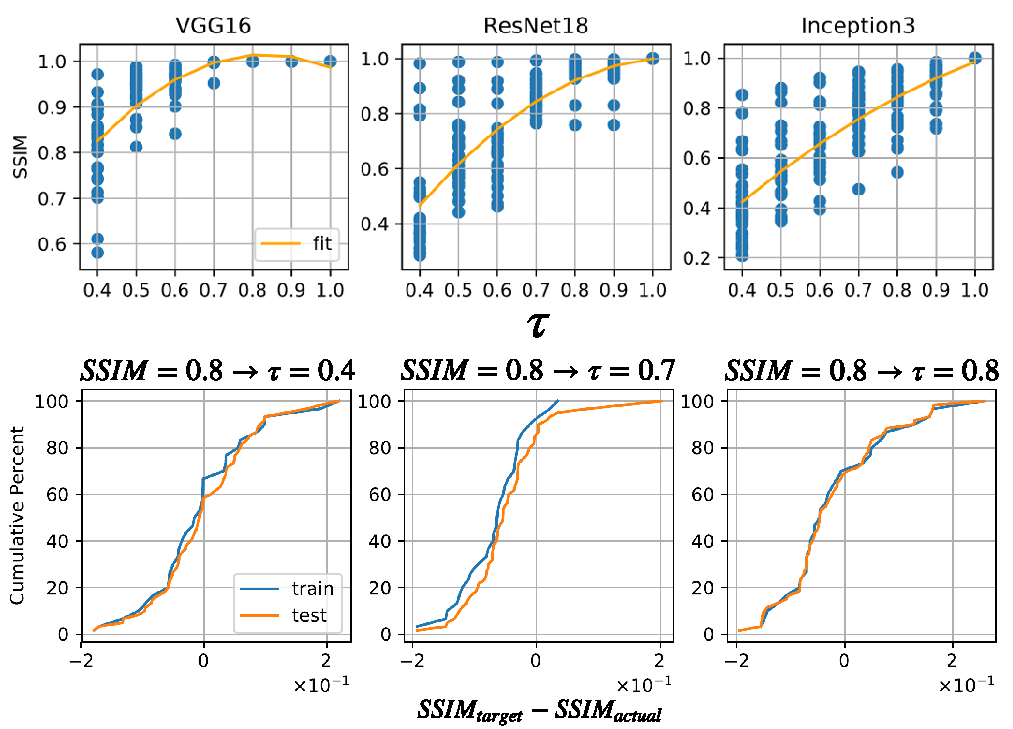
\includegraphics[width=\columnwidth]{images/system_tuning}
\caption{(a) SSIM variation and degree two curve fit for a sample of OCT dataset. (b) CDF plot for the SSIM deviation for the $\tau$ values picked from the curve fit for a target SSIM of 0.9.}
\label{fig:system_tuning}
\end{figure}

% \begin{figure}[t]
% 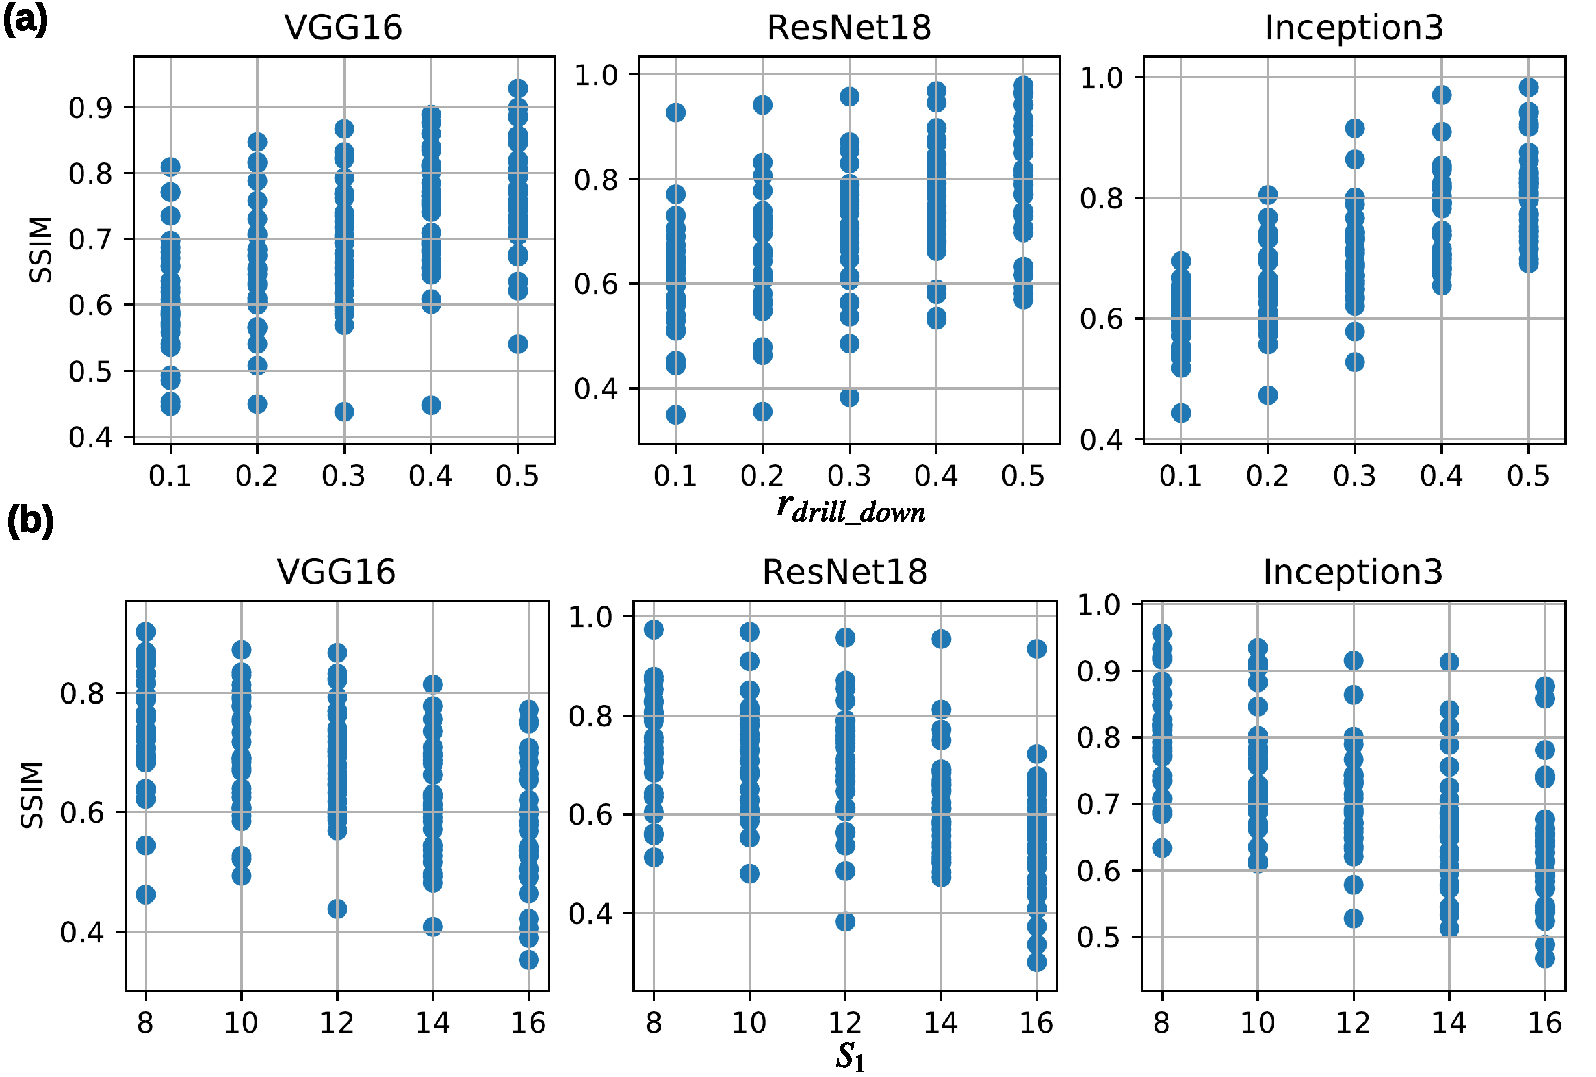
\includegraphics[width=\columnwidth]{images/adaptive_ssim}
% \caption{(a) SSIM variation for changing $r_{drill\_down}$ fixing $\tau=1$, $S_1=12$, and $S_2=4$. (b) SSIM variation for changing $S_1$ fixing $\tau=1.0$, $S_2=4$, and $r_{drill\_down}=0.3$ for a sample $(n=30)$ of OCT dataset.}
% \label{fig:adaptive_ssim}
% \end{figure}

